\section{Fejlesztői dokumentáció}
\subsection{Megoldási terv}
A rendszer több különálló modulból kell hogy álljon:
\begin{itemize}
\item Felhasználói weboldal, ahol a bejelentkezést végre akarják hajtani. Jelen esetben ez egy JavaEE backend (Spring Framework), és AngularJS frontendet használó alkalmazás. Ennek az alkalmazásnak a bejelentkezési mechanizmusa kell , hogy össze legyen integrálva az E-Group IDX szerverével. Erről az integrálásról a megvalósítás pontban írok részletesebben. Ez az oldal pusztán demonstrálásra lesz használva, egy publikus oldalról gesztikuláció alapú bejelentkezéssel egy védett oldalt lehet majd elérni, amely kiírja az azonosított felhasználó nevét. Kijelentkezés menüpont pedig bontja a munkamenetet.
\item Az E-Group IDX szervere, amelyben új modulként jelenik meg a gesztikuláció alapú bejelentkezés. Mivel a jelenlegi modulok hasonló, off-site kommunikációt egy kivételével nem tartalmaznak, így a jelenlegi limitáló tényezők miatt szükséges lesz egy authentikáló alkalmazásra is, amit az IDX szerver REST hívásokon keresztül el tud érni. A lényeges logika ebben a rendszerben kell megvalósuljon, ám a felhasználókról semmilyen adatot nem tartalmazhat permanensen.
\item Authentikáló alkalmazás, amely a belépési logikát tartalmazza. Egy IDX felületről indított bejelentkezésről REST-en keresztül üzenetet kell kapnia, majd ezt az rekordot társítani kell tudni egy a mobil alkalmazásból jövő üzenettel. A mobil alkalmazás üzenetei és az IDX szerverből érkező perzisztált rekord alapján valamilyen logika mentén a bejelentkezést el kell fogadnia vagy el kellutasítania. Ezt az üzenetet nem küldheti vissza az IDX szervernek, ehelyett user interakció vagy esetleges pollozó algoritmus kell lekérdezze tőle.
\item Mobil alkalmazás, amely támogatja a regisztrációt és a bejelentkezést. Ez az alkalmazás az IDX vagy a felhasználói weboldal felületéről kell indítható legyen, innen megfelelő kezdeti paramétereketkell fogadnia, ami segítségével tudnia kell, hogy regisztráció illetve bejelentkezés esetén hova továbbítsa a feldolgozott adatokat.
\item Egy vagy több third party arcfelismerő alkalmazás, amely hosszútávon lehet egy online, illetve offline megoldás is, beépítésekor törekedni kell a könnyű konfigurációra. Az authentikáló alkalmazás fogja hívni a bejelentkezés megfelelő lépéseiben, a válasz alapján lehet eldönteni a bejelentkezés sikerességét. Jelenleg a Microsoft Project Oxford és a Face++ kerül beépítésre
\end{itemize}

Az alábbi ábra mutatja a rendszer komponenseit és azok kommunikációját. Az egyenes nyíl jelzi, ha az adott komponens meg tudja szólítani valamilyen módon a célkomponenst. A kérésre adott választ nem jelöltem.

\begin{figure}[h]
 \begin{minipage}{1\textwidth} 
\centering
    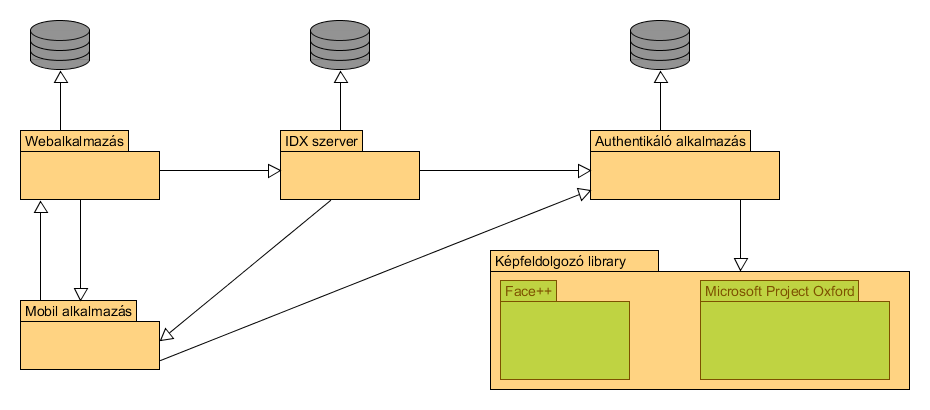
\includegraphics[scale=0.47]{img/rendszerkomponensek}
    \caption{A rendszer komponensei}
 \end{minipage}
\end{figure}

\subsubsection{Felhasználó weboldal}
A publikus főoldalon van lehetőségünk bejelentkezni, illetve amennyiben még nincsen felhasználónk, regisztrálni. A bejelentkezés gombra kattintva megfelelő IDX integráció esetén az IDX bejelentkező felületére leszünk továbbítva. Regisztráció esetén egy felhasználónév megadásával indíthatunk új folyamatot. Itt ellenőrizni kell a felhasználónév szabad felhasználást, illetve mivel itt még csak paramétereket generálunk a mobilalkalmazásnak, a regisztrációs adatok csak később kerülnek adatbázisba, így ezt később is ellenőrizni kell!

\begin{sidewaysfigure}
\centering

         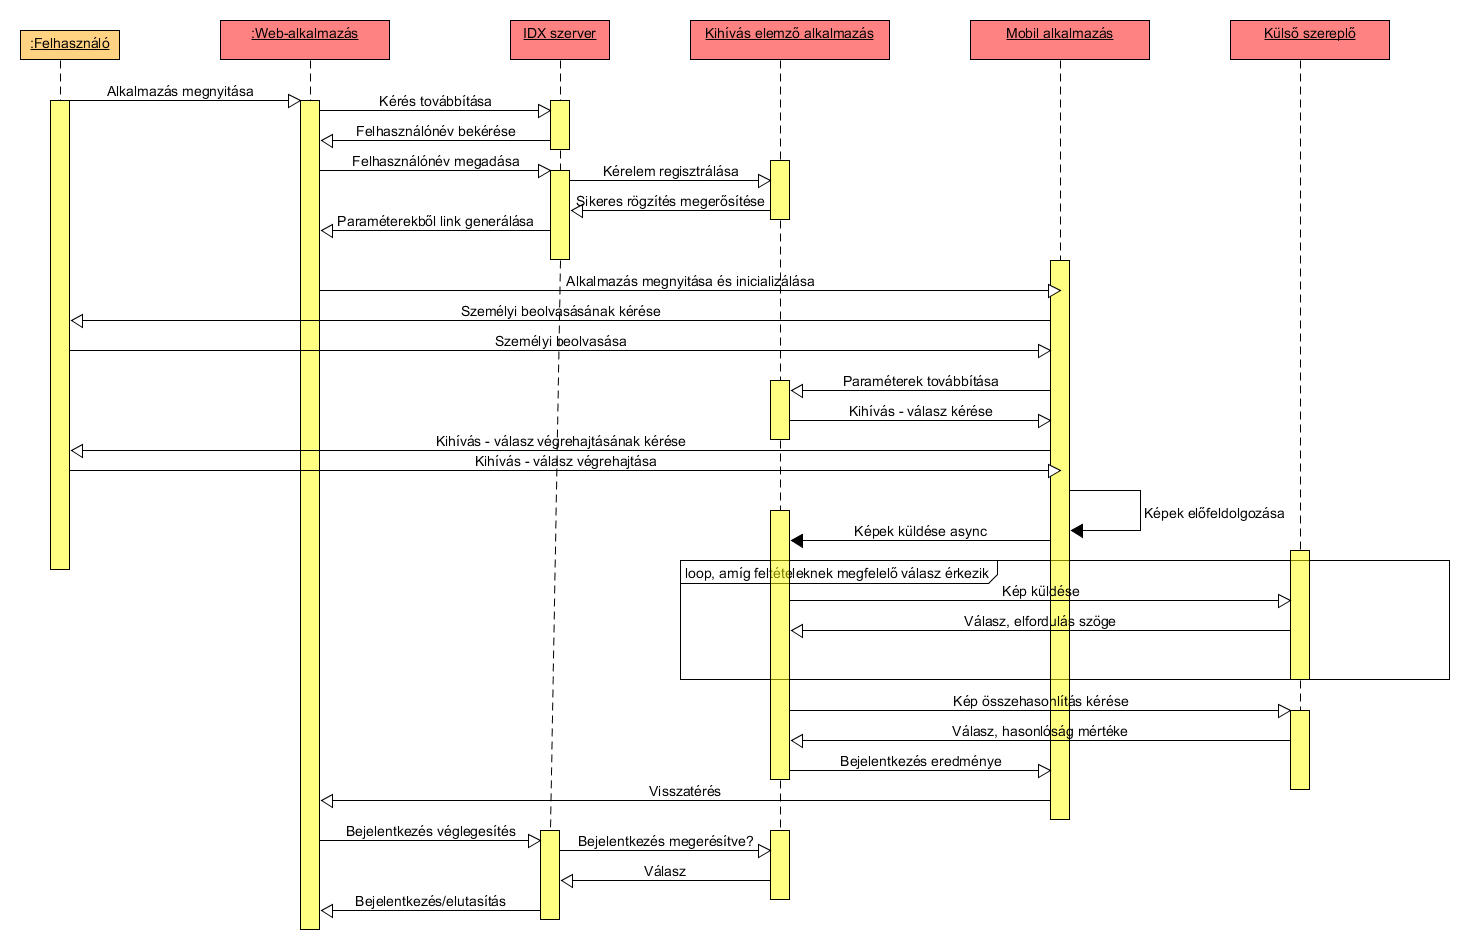
\includegraphics[scale=0.47]{img/szekvencia}

    \caption{Bejelentkezés szekvencia diagramja}
\end{sidewaysfigure}